%\documentclass{minimal}
%\usepackage[pdftex,active,tightpage]{preview}
%\usepackage{tikz}
%\begin{document}
%\begin{preview}
%%%%%%%%%%%%%%%%%%%%%%%%%%%%%%
	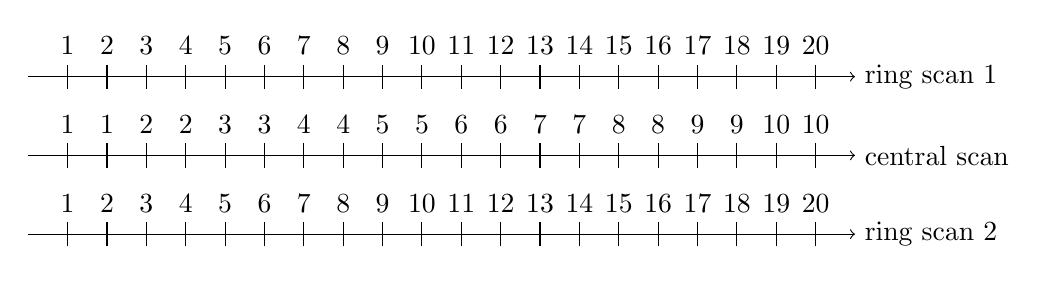
\begin{tikzpicture}[scale=0.5]
	%
	\def\linegap{2}%1.6181229773462783171521035598706}
	\def\length{20}
	\def\centrallength{10}
	\def\ticklength{.309}
	% lines
		\foreach \y/\label in {0/central scan,\linegap/ring scan 1,-\linegap/ring scan 2}%
			\draw [->] (0,\y) -- (\length+1,\y) node [anchor=west] {\label};
	% central scan		
		\foreach \x in {1,...,\centrallength}
			\draw (2*\x-1,0-\ticklength) -- (2*\x-1,0+\ticklength) node [anchor=south] {\x}
				(2*\x,0-\ticklength) -- (2*\x,0+\ticklength) node [anchor=south] {\x};
	% ring scan on top
		\foreach \y in {1,...,\length}
			\draw (\y,\linegap-\ticklength) -- (\y,\linegap+\ticklength) node [anchor=south] {\y};
%	% ring scan on bottom
		\foreach \z in {1,...,\length}
			\draw (\z,-\linegap-\ticklength) -- (\z,-\linegap+\ticklength) node [anchor=south] {\z};
	\end{tikzpicture}
%%%%%%%%%%%%%%%%%%%%%%%%%%%%%%
%\end{preview}
%\end{document}